\section{Respuesta en Frecuencia}

\subsection{Diagramas de Bode}
En este apartado se generaron con el osciloscopio los diagramas de bode correspondientes a la salida de voltaje de los diferentes elementos.
Inicialmente tenemos el diagrama de bode correspondiente a la salida de tensión sobre el inductor que se puede ver en el gráfico de la Figura \ref{fig:bode_inductor}. 

\begin{figure}[H]
\centering
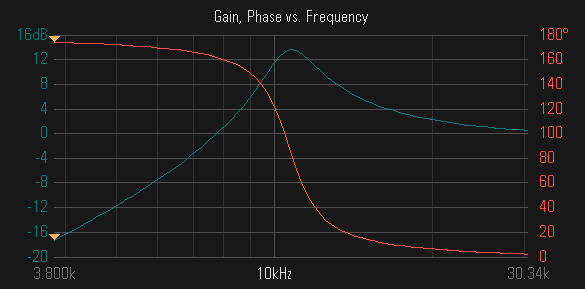
\includegraphics[width=1\textwidth]{Bode_L.png}
\caption{Diagrama de Bode experimental para la salida sobre el inductor.}
\label{fig:bode_inductor}
\end{figure}

Luego esta el diagrama de bode correspondiente a la salida de tensión sobre la resistencia que se puede ver en el gráfico de la Figura \ref{fig:bode_resistencia}. 

\begin{figure}[H]
\centering
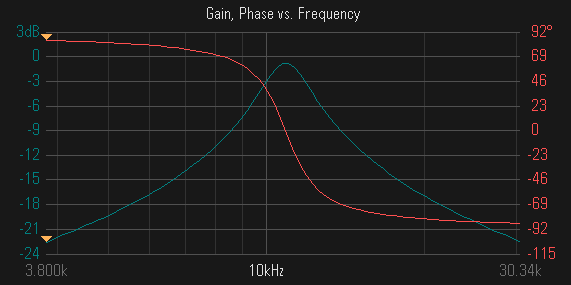
\includegraphics[width=1\textwidth]{Bode_R.png}
\caption{Diagrama de Bode experimental para la salida sobre la resistencia.}
\label{fig:bode_resistencia}
\end{figure}

Por ultimo el diagrama de bode correspondiente a la salida de tensión sobre el capacitor que se puede ver en el gráfico de la Figura \ref{fig:bode_capacitor}. 

\begin{figure}[H]
\centering
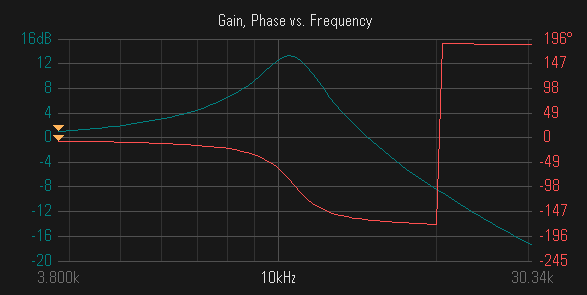
\includegraphics[width=1\textwidth]{Boede_Capacitor.png}
\caption{Diagrama de Bode experimental para la salida sobre el capacitor.}
\label{fig:bode_capacitor}
\end{figure}


\subsection{Mediciones puntuales del diagrama de Bode}

Para complementar los diagramas de Bode obtenidos experimentalmente, se realizaron mediciones puntuales de amplitud y fase para la salida sobre el inductor. En las tablas se comparan los valores experimentales con los obtenidos mediante simulación para los tres rangos de frecuencia solicitados.

En el Cuadro \ref{tab:bode_inductor_fmenos1_f1} se pueden ver los datos obtenidos de los 5 puntos elegidos de manera experimental y utilizando la simulación.

\begin{table}[H]
\centering
\caption{Mediciones puntuales del Bode del inductor entre \(f_{-1}\) y \(f_1\).}
\label{tab:bode_inductor_fmenos1_f1}
\resizebox{\textwidth}{!}{
\begin{tabular}{c c c c c c c c c}
\toprule
\multirow{2}{*}{Punto} 
& \multicolumn{4}{c}{Medición experimental}
& \multicolumn{4}{c}{Simulación} \\
\cmidrule(lr){2-5} \cmidrule(lr){6-9}
& \(f\,[\si{\kilo\hertz}]\)
& \(\Delta \varphi\,[^\circ]\)
& \(V_{\text{in}}\,[\si{\volt}_{pp}]\)
& \(V_{\text{out}}\,[\si{\volt}_{pp}]\)
& \(f\,[\si{\kilo\hertz}]\)
& \(\Delta \varphi\,[^\circ]\)
& \(V_{\text{in}}\,[\si{\volt}]\)
& \(V_{\text{out}}\,[\si{\volt}]\) \\
\midrule
1 & 8  & 162 & 1,05 & 1,25 & 8  & 155 & 1 & 0,866 \\
2 & 10 & 119 & 1,05 & 3,94 & 10 & 140 & 1 & 1,264 \\
3 & 11 & 68  & 1,03 & 4,62 & 11 & 123 & 1 & 1,525 \\
4 & 12 & 39  & 1,05 & 3,54 & 12 & 93  & 1 & 1,763 \\
5 & 14 & 18  & 1,05 & 2,29 & 14 & 39  & 1 & 1,618 \\
\bottomrule
\end{tabular}
}
\end{table}

Luego en el cuadro \ref{tab:bode_inductor_fmenos2_fmenos1} se pueden ver los datos correspondientes a los puntos elegidos en el rango entre \(f_{-2}\) y \(f_{-1}\).

\begin{table}[H]
\centering
\caption{Mediciones puntuales del Bode del inductor entre \(f_{-2}\) y \(f_{-1}\).}
\label{tab:bode_inductor_fmenos2_fmenos1}
\resizebox{\textwidth}{!}{
\begin{tabular}{c c c c c c c c c}
\toprule
\multirow{2}{*}{Punto} 
& \multicolumn{4}{c}{Medición experimental}
& \multicolumn{4}{c}{Simulación} \\
\cmidrule(lr){2-5} \cmidrule(lr){6-9}
& \(f\,[\si{\kilo\hertz}]\)
& \(\Delta \varphi\,[^\circ]\)
& \(V_{\text{in}}\,[\si{\volt}_{pp}]\)
& \(V_{\text{out}}\,[\si{\volt}_{pp}]\)
& \(f\,[\si{\kilo\hertz}]\)
& \(\Delta \varphi\,[^\circ]\)
& \(V_{\text{in}}\,[\si{\volt}]\)
& \(V_{\text{out}}\,[\si{\volt}]\) \\
\midrule
1 & 7   & 169 & 1,05 & 0,80 & 7   & 158 & 1 & 0,720 \\
2 & 7,5 & 160 & 1,05 & 1,01 & 7,5 & 157 & 1 & 0,790 \\
\bottomrule
\end{tabular}
}
\end{table}

Finalmente en el Cuadro \ref{tab:bode_inductor_f1_f2} se puede ver los datos de los puntos elegidos en el intervalo entre \(f_1\) y \(f_2\).
\begin{table}[H]
\centering
\caption{Mediciones puntuales del Bode del inductor entre \(f_1\) y \(f_2\).}
\label{tab:bode_inductor_f1_f2}
\resizebox{\textwidth}{!}{
\begin{tabular}{c c c c c c c c c}
\toprule
\multirow{2}{*}{Punto} 
& \multicolumn{4}{c}{Medición experimental}
& \multicolumn{4}{c}{Simulación} \\
\cmidrule(lr){2-5} \cmidrule(lr){6-9}
& \(f\,[\si{\kilo\hertz}]\)
& \(\Delta \varphi\,[^\circ]\)
& \(V_{\text{in}}\,[\si{\volt}_{pp}]\)
& \(V_{\text{out}}\,[\si{\volt}_{pp}]\)
& \(f\,[\si{\kilo\hertz}]\)
& \(\Delta \varphi\,[^\circ]\)
& \(V_{\text{in}}\,[\si{\volt}]\)
& \(V_{\text{out}}\,[\si{\volt}]\) \\
\midrule
1 & 22,5 & 3 & 1,05 & 1,33 & 22,5 & 8 & 1 & 1,150 \\
2 & 27,5 & 1,5 & 1,05 & 1,25 & 27,5 & 6 & 1 & 1,096 \\
\bottomrule
\end{tabular}
}
\end{table}

\newpage